\documentclass[11pt]{article}
\usepackage[margin = 1in]{geometry}
\usepackage{amsmath}
\usepackage{amssymb}
\usepackage{amsthm}
\usepackage{graphicx}
\usepackage{url}
\usepackage[parfill]{parskip}
\usepackage{listings}
\usepackage{caption}
\usepackage{subcaption}
\usepackage[utf8]{inputenc}
\usepackage{xcolor}
\definecolor{codegreen}{rgb}{0,0.6,0}
\definecolor{codegray}{rgb}{0.5,0.5,0.5}
\definecolor{codepurple}{rgb}{0.58,0,0.82}
\definecolor{backcolour}{rgb}{0.95,0.95,0.92}
\lstdefinestyle{mystyle}{
	backgroundcolor=\color{backcolour},   
	commentstyle=\color{codegreen},
	keywordstyle=\color{magenta},
	numberstyle=\tiny\color{codegray},
	stringstyle=\color{codepurple},
	basicstyle=\ttfamily\footnotesize,
	breakatwhitespace=false,         
	breaklines=true,                 
	captionpos=b,                    
	keepspaces=true,                 
	numbers=left,                    
	numbersep=5pt,                  
	showspaces=false,                
	showstringspaces=false,
	showtabs=false,                  
	tabsize=2
}
\lstset{style=mystyle}
\newcommand{\skipline}{\vspace{\baselineskip}}
\newcommand{\spacer}{\noalign{\medskip}}
\newcommand{~}{\sim}
\newcommand{\approches}{\rightarrow}
\newcommand{\qarrow}{\quad \rightarrow \quad}
\newcommand{\qqarrow}{\qquad \rightarrow \qquad}
\newcommand{\qtext}[1]{\quad \text{ #1 } \quad}
\newcommand{\qqtext}[1]{\qquad \text{ #1 } \qquad}
\newcommand{\pard}[2]{\frac{\partial #1}{\partial #2}}
\newcommand{\answer}[1]{\textbf{\boldmath #1}}
\newenvironment{problem}[1]{\textbf{Problem #1: }}{\newpage}

\begin{document}
	\begin{center}
		\textbf{Chess AI Logic} \\
		\textbf{Stephen Giang} \\
		\skipline \skipline
	\end{center}

	The goal of this Chess AI is to be able to make accurate chess moves based on the points value system (PVS), position, and depth.
	\newpage
	\text{}
	\begin{figure}[h!]
		\centering
		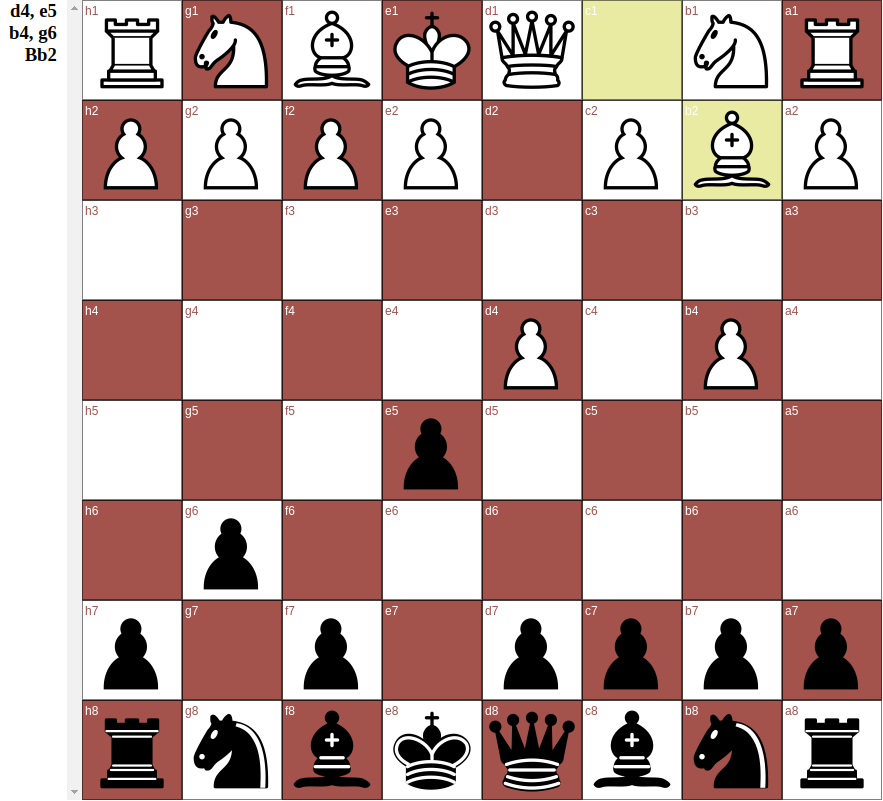
\includegraphics[width=.8\linewidth]{example1}
	\end{figure}
	\\
	Notice the logic of an AI based off purely the points value system and only being able to see one move ahead in depth. Because of the PVS, we can take a look at the black pawn at E5 and the black bishop on F8.  All other pieces don't have moves that can capture another piece, which would lead to a non positive net return in points. 
	\\ \\
	If the black pawn at E5 takes the white pawn at D4, this would give that move a return of positive one.  Looking forward at a depth of one, the white side would then use either the Queen or bishop on B2 to take the black pawn now on D4 to equalize their previous return of -1.  In this case, the white side should use the bishop for the reason that we want to reward taking larger value pieces with smaller value pieces, as this contains less risk. Thus, this would lead to a net return of 0. If we were to look at how position comes into play, moving the black pawn doesn't really give us more moves to choose from, if anything, the other side has more moves and more chance to take black's pieces.  So this should lead to a negative position value. 
	\\ \\
	If the black bishop at F8 takes the white pawn at B4, this would give that move a return of positive one.  Looking forward at a depth of one, the white side would not be able to take that bishop or any other pieces for that matter as it is forced to block the king with its pieces.  Thus, this would lead to a net return of 1.  In terms of position, moving the black bishop, allows it to put white into check, limiting white's possible moves.  This should lead to a positive value. 
	\\ \\
	The best move assuming only using the PVS and a depth of 1 would be Bxb4.
	
\end{document}
